\section{Basic document structure}

Next, we explore abstracts and how to partition a \LaTeX\ document into different chapters, sections and paragraphs.

\subsection{Abstracts}

Scientific articles usually provide an \emph{abstract} which is a brief overview/summary of their core topics, or arguments. The next example demonstrates typesetting an abstract using \LaTeX’s abstract environment:

\begin{tcolorbox}
\begin{verbatim}
    \documentclass{article}
    \begin{document}
    \begin{abstract}
    This is a simple paragraph at the beginning of the 
    document. A brief introduction about the main subject.
    \end{abstract}
    \end{document}
\end{verbatim}
\end{tcolorbox}

This example produces the following output:

\begin{mdframed}
    \begin{abstract}
    This is a simple paragraph at the beginning of the document. A brief introduction about the main subject.
    \end{abstract}
\end{mdframed}

\subsection{Paragraphs and new lines}

With the abstract in place, we can begin writing our first paragraph. The next example demonstrates:

\begin{itemize}
    \item how a new paragraph is created by pressing the "enter" key twice, ending the current line and inserting a subsequent blank line;
    \item how to start a new line without starting a new paragraph by inserting a manual line break using the \verb|\\| command, which is a double backslash; alternatively, use the \verb|\newline| command.
\end{itemize}

The third paragraph in this example demonstrates use of the commands \verb|\\| and \verb|\newline|:

\begin{tcolorbox}
\begin{verbatim}
    \documentclass{article}
    \begin{document}

    \begin{abstract}
    This is a simple paragraph at the beginning of the 
    document. A brief introduction about the main subject.
    \end{abstract}

    After our abstract we can begin the first paragraph, then 
    press ``enter'' twice to start the second one.

    This line will start a second paragraph.

    I will start the third paragraph and then add \\ a manual 
    line break which causes this text to start on a new line 
    but remains part of the same paragraph. Alternatively, I 
    can use the \verb|\newline|\newline command to start a 
    new line, which is also part of the same paragraph.
    \end{document}
\end{verbatim}
\end{tcolorbox}

This example produces the following output:

\begin{mdframed}
    \begin{abstract}
    This is a simple paragraph at the beginning of the document. A brief introduction about the main subject.
    \end{abstract}

    \-\hspace{20pt}After our abstract we can begin the first paragraph, then press ``enter'' twice to start the second one.

    \-\hspace{20pt}This line will start a second paragraph.

    \-\hspace{20pt}I will start the third paragraph and then add \\ a manual line break which causes this text to start on a new line but remains part of the same paragraph. Alternatively, I can use the \verb|\newline|\newline command to start a new line, which is also part of the same paragraph.
\end{mdframed}

Note how \LaTeX\ automatically indents paragraphs—except immediately after document headings such as section and subsection—\href{https://www.overleaf.com/learn/latex/Learn_LaTeX_in_30_minutes#Chapters_and_sections}{as we will see}.

New users are advised that multiple \verb|\\| or \verb|\newlines| should not used to “simulate” paragraphs with larger spacing between them because this can interfere with \LaTeX’s typesetting algorithms. The recommended method is to continue using blank lines for creating new paragraphs, without any \verb|\\|, and load the \href{https://ctan.org/pkg/parskip?lang=en}{parskip package} by adding \verb|\usepackage{parskip}| to the preamble.

Further information on paragraphs can be found in the following articles:

\begin{itemize}
    \item \href{https://www.overleaf.com/learn/latex/Paragraphs_and_new_lines}{Paragraphs and new lines}
    \item \href{https://www.overleaf.com/learn/latex/Articles/How_to_change_paragraph_spacing_in_LaTeX}{How to change paragraph spacing in LaTeX}
    \item \href{https://www.overleaf.com/learn/latex/Errors/LaTeX_Error%3A_There%27s_no_line_here_to_end}{LaTeX Error: There's no line here to end} provides additional advice and guidance on using \verb|\\|.
\end{itemize}

\subsection{Chapters and sections}

Longer documents, irrespective of authoring software, are usually partitioned into parts, chapters, sections, subsections and so forth. LaTeX also provides document-structuring commands but the available commands, and their implementations (what they do), can depend on the document class being used. By way of example, documents created using the book class can be split into parts, chapters, sections, subsections and so forth but the \verb|letter| class does not provide (support) any commands to do that.

This next example demonstrates commands used to structure a document based on the \verb|book| class:

\begin{tcolorbox}
\begin{verbatim}
    \documentclass{book}
    \begin{document}

    \chapter{First Chapter}

    \section{Introduction}

    This is the first section.

    Lorem  ipsum  dolor  sit  amet,  consectetuer  adipiscing  
    elit. Etiam  lobortisfacilisis sem.  Nullam nec mi et 
    neque pharetra sollicitudin.  Praesent imperdietmi nec ante. 
    Donec ullamcorper, felis non sodales...

    \section{Second Section}

    Lorem ipsum dolor sit amet, consectetuer adipiscing elit.  
    Etiam lobortis facilisissem.  Nullam nec mi et neque pharetra 
    sollicitudin.  Praesent imperdiet mi necante...

    \subsection{First Subsection}
    Praesent imperdietmi nec ante. Donec ullamcorper, felis non 
    sodales...

    \section*{Unnumbered Section}
    Lorem ipsum dolor sit amet, consectetuer adipiscing elit.  
    Etiam lobortis facilisissem...
    \end{document}
\end{verbatim}
\end{tcolorbox}

This example produces the following output:

\fbox{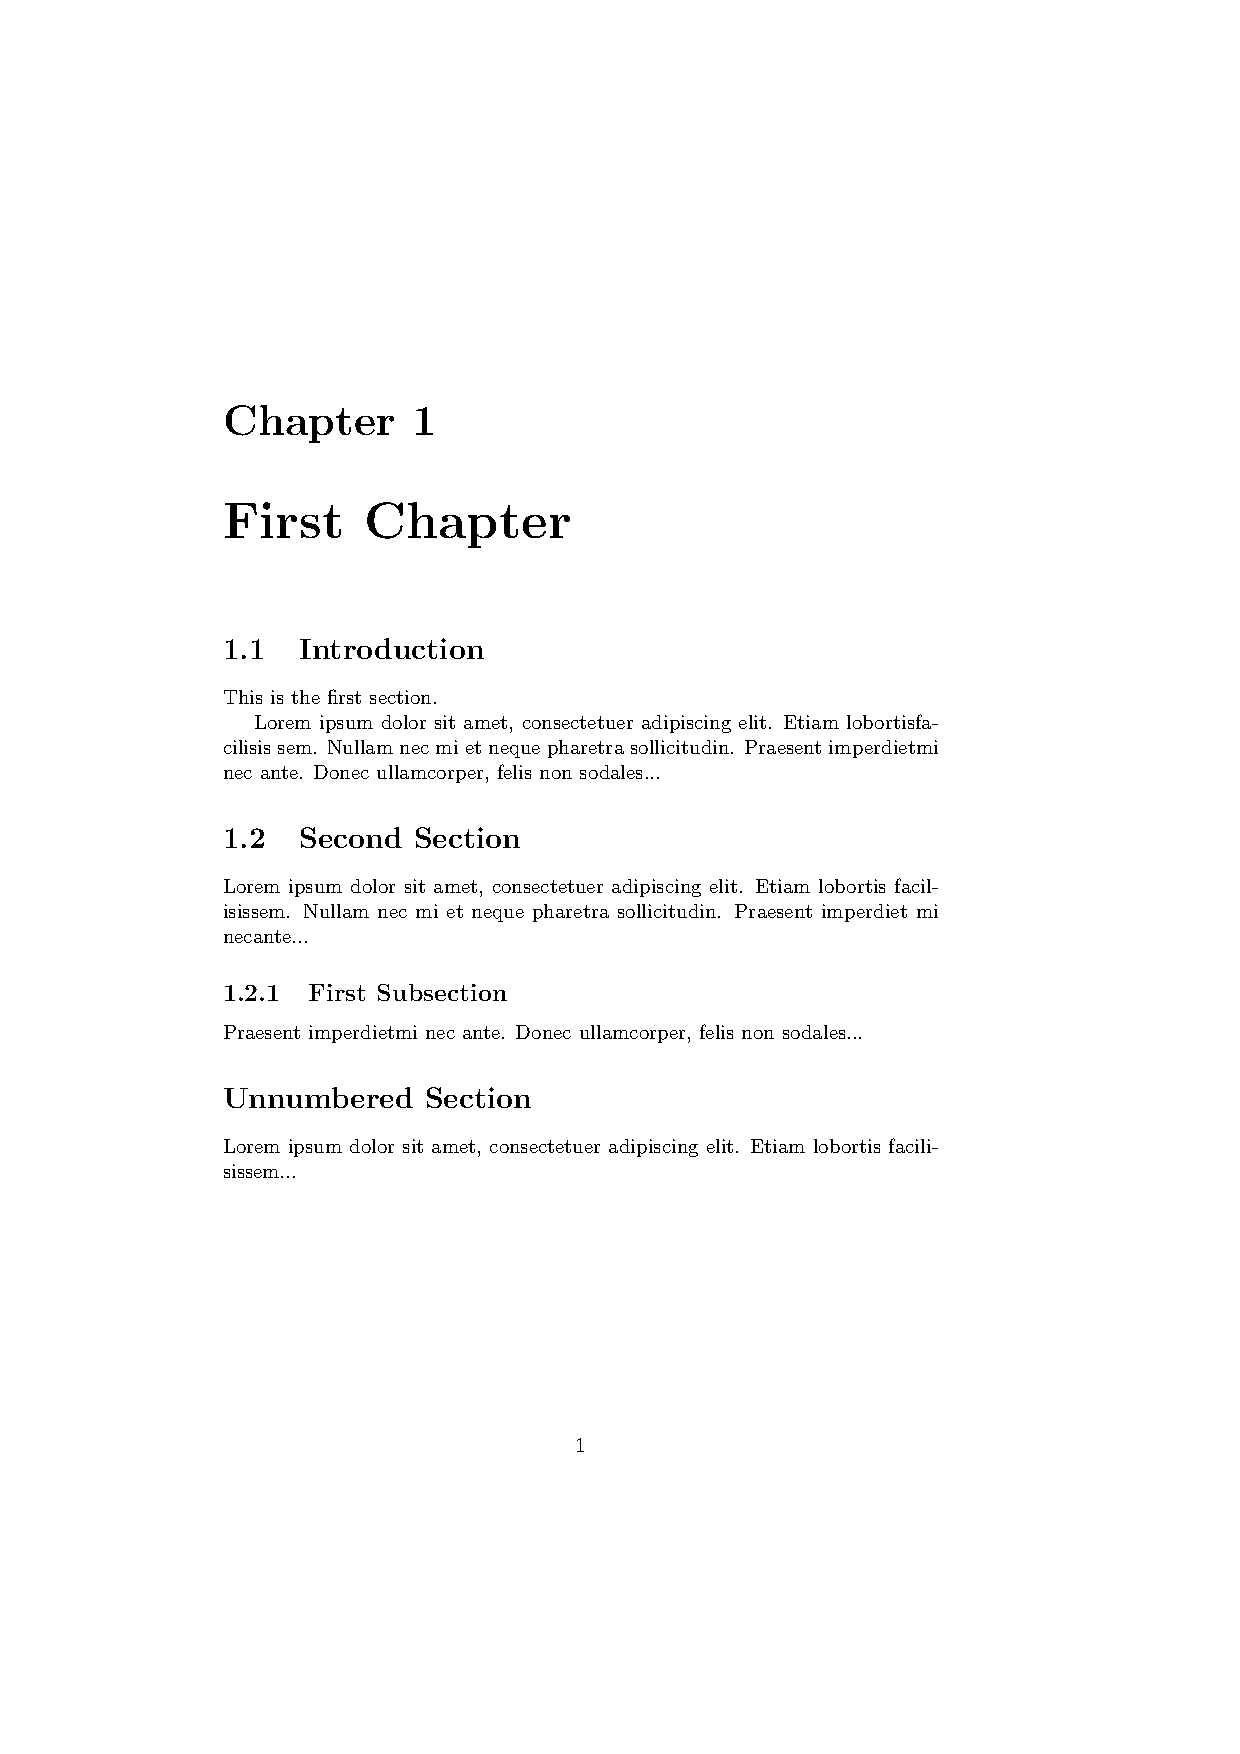
\includegraphics[width=\textwidth]{Example 12-1.pdf}}

The names of sectioning commands are mostly self-explanatory; for example,\\ \verb|\chapter{First Chapter}| creates a new chapter titled \verb|First Chapter|,\\\verb|\section{Introduction}| produces a section titled \verb|Introduction|, and so forth. Sections can be further divided into \verb|\subsection{...}| and even \verb|\subsubsection{...}|. The numbering of sections, subsections etc. is automatic but can be disabled by using the so-called \emph{starred version} of the appropriate command which has an asterisk (\verb|*|) at the end, such as \verb|\section*{...}| and \verb|\subsection*{...}|.

\emph{Collectively}, LaTeX document classes provide the following sectioning commands, with specific classes each supporting a relevant subset:

\begin{itemize}
    \item \verb|\part{part}|
    \item \verb|\chapter{chapter}|
    \item \verb|\section{section}|
    \item \verb|\subsection{subsection}|
    \item \verb|\subsubsection{subsubsection}|
    \item \verb|\paragraph{paragraph}|
    \item \verb|\subparagraph{subparagraph}|
\end{itemize}

In particular, the \verb|\part| and \verb|\chapter| commands are only available in the \verb|report| and \verb|book| document classes.

Visit the \href{https://www.overleaf.com/learn/latex/Sections_and_chapters}{Overleaf article about sections and chapters} for further information about document-structure commands.